\begin{frame}
\frametitle{Architecture}
\framesubtitle{Choix des cartes}
\begin{description}
	\item [Quelle carte choisir ?]
	\item Réunion Brainstorming;
	\item Énumération des avantages et désavantages;
	\item Facilité de mise en place et programmation;
	\item Budget.
\end{description}
\end{frame}

\begin{frame}
\frametitle{Architecture}
\framesubtitle{Arduino}
\begin{description}
	\item [Avantages]
	\item Temps réel (ATmega328 8 bits d'Atmel à 16MHz);
	\item Communautaire et très documenté sur internet;
	\item Programmation aisée en C++.
	\item [Désavantages]
	\item 32 Ko d'espace mémoire;
	\item Impossibilité d'intégrer le module caméra avec Arduino.
\end{description}
\end{frame}

\begin{frame}
\frametitle{Architecture}
\framesubtitle{Raspberry Pi}
\begin{description}
	\item [Avantages]
	\item Utilisation facile, architecture linux;
	\item Utilisation de la caméra aisée;
	\item OpenCV, très bien documenté.
	\item [Désavantages]
	\item Limitation nombre pins, besoin d'une carte supplémentaire;
	\item Système exploitation, implique que l'on est pas en temps réel; 
	\item Elle freeze (Testé en laboratoire).
\end{description}
\end{frame}

\begin{frame}
\frametitle{Architecture}
\framesubtitle{DE0 nano}
\begin{description}
	\item [Avantages]
	\item Instantané;
	\item Carte plus performante que les autres;
	\item Nombreuses pins à disposition.
	\item [Désavantages]
	\item Difficulté lors de la programmation (VHDL);
	\item Coût important.
\end{description}
\end{frame}

\begin{frame}
\frametitle{Architecture}
\framesubtitle{Buts principaux}
Architecture modulable s'articulant autour de 4 modules principaux :
\begin{itemize}
	\item Arduino Master, gestion de l'ensemble des modules ;
	\item Arduino Motor, gestion des moteurs avec régulation ;
	\item Raspberry Pi, définition des objectifs à atteindre ;
	\item Arduino Bras, gestion de la pince.
\end{itemize}
\end{frame}

\begin{frame}
\frametitle{Architecture}
\framesubtitle{Schéma bloc hardware}
\begin{figure}[!ht]
	\centering
	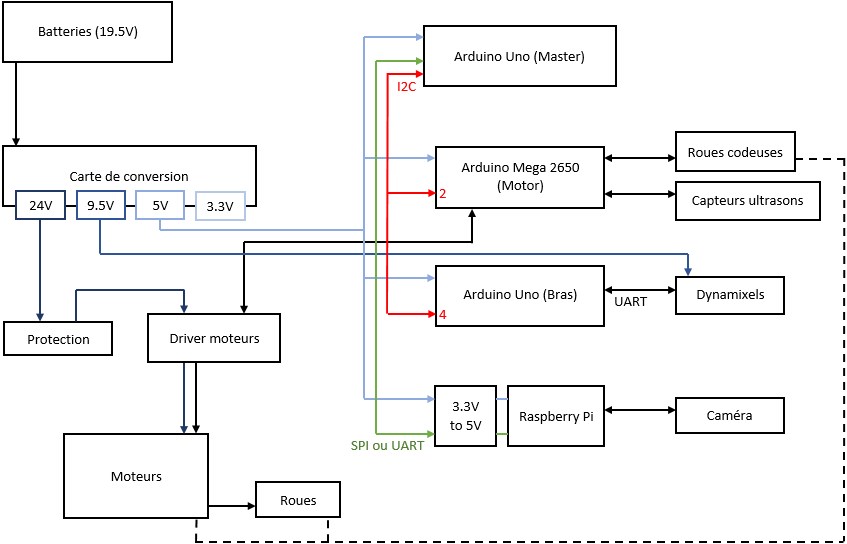
\includegraphics[scale=0.45]{hardware.PNG}
	\caption{Schéma bloc hardware}
\end{figure}
\end{frame}